\documentclass[10pt]{article}
\usepackage[utf8]{inputenc}

% Any additional packages needed should be included after jmlr2e.
% Note that jmlr2e.sty includes epsfig, amssymb, natbib and graphicx,
% and defines many common macros, such as 'proof' and 'example'.

\usepackage{jmlr2e}
\usepackage[a4paper, right=2.5cm, left=2.5cm, bottom=2.5cm, top=3cm]{geometry}
\usepackage{amsmath, mathtools}
\usepackage{booktabs}
\usepackage{algpseudocode}
\usepackage{algorithm}
\usepackage{float}
\usepackage{subfloat}
\usepackage{caption}
\usepackage{subcaption}
\graphicspath{{../images/}}
\usepackage{xcolor}
\usepackage{tikz}
\usetikzlibrary{bayesnet}
\usetikzlibrary{arrows}
\usepackage{hyperref}


% Definitions of handy macros can go here
\newcommand{\fracpartial}[2]{\frac{\partial #1}{\partial  #2}}
\newcommand{\prob}{\mathbb{P}} 
\newcommand{\R}{\mathbb{R}}
\newcommand{\N}{\mathbb{N}}
\newcommand{\E}{\mathbb{E}}
\renewcommand{\O}{\mathcal{O}}
\renewcommand{\L}{\mathcal{L}}
\newcommand{\eps}{\varepsilon}
\newcommand{\dd}{\, \mathrm{d}}
\newcommand{\J}{\mathcal{J}}
\DeclareMathOperator*{\argmin}{arg\,min}
\DeclareMathOperator*{\argmax}{arg\,max}
\DeclareMathOperator*{\minimize}{minimize}
\DeclareMathOperator*{\KL}{KL}
\newcommand{\intset}[2]{\{#1, ..., #2\}}
\newcommand{\mnbs}{\nobreak\hspace{.16667em}}


% Heading arguments are {volume}{year}{pages}{submitted}{published}{author-full-names}
% \jmlrheading{}{}{}{}{}{Bastien LE CHENADEC, SOFIANE EZZEHI and THEILO TERRISSE}

% Short headings should be running head and authors last names

\ShortHeadings{Mixture Models for Community Detection}{B. LE CHENADEC, S. EZZEHI and T. TERRISSE}
\firstpageno{1}

\begin{document}

\title{Mixture Models for Community Detection}

\author{\name Bastien Le Chenadec \email bastien.le-chenadec@eleves.enpc.fr \\
    \addr Ecole des Ponts Paristech
    \AND
    \name Sofiane Ezzehi \email sofiane.ezzehi@eleves.enpc.fr \\
    \addr Ecole des Ponts Paristech
    \AND
    \name Theïlo Terrisse \email theilo.terrisse@eleves.enpc.fr \\
    \addr Ecole des Ponts Paristech
}

\maketitle

\textcolor{red}{Quelques remarques:
    \begin{itemize}
        \item hésitez pas à utiliser Zotero pour exporter d'éventuelles références bibliographiques, histoire d'avoir un remplissage uniforme e de gagner du temps
        \item Une fois une abbréviation introduite (ex: SBM), si possible toujours utiliser l'abbréviation et ne pas ré-écrire l'expression entière
        \item Je propose de préférer le terme de "cluster" à "community".
    \end{itemize}
}

\begin{contribstatement}
    TODO
\end{contribstatement}

% \begin{keywords}
%   Mixture Models, Graph Clustering, Community Detection, EM algorithm
% \end{keywords}

\section{Introduction}

Garph clustering, also referred to as ``community detection'' \cite{fortunato_community_2010}, is the problem of revealing clusters within a graph where a ``cluster'' is often defined as a set of nodes that are more densely connected between them than with the rest of the network.
More precisely, a cluster $C$ is defined as a group of nodes with an internal density $\delta_{int}(C)$ larger than its inter-community density $\delta_{ext}(C)$, where
\begin{equation}
    \delta_{int} = \frac{\text{\# internal edges of }C}{n_C (n_C - 1) / 2} \quad \text{and} \quad \delta_{ext} = \frac{\text{\# inter-cluster edges of C}}{n_C (n - n_C)}
\end{equation}
with $n$ the number of nodes of the graph, $n_C$ the number of nodes in the cluster $C$ and internal (resp. inter-cluster) edges are edges between nodes of $C$ (resp. between nodes of $C$ and nodes outside of $C$). This definition is actually characteristic of homophilious clusters, while heterophilious clusters would be such that $\delta_{int}(C) < \delta_{ext}(C)$.
Graph clustering has tremendous applications in the study of real networks such as
social [1] or biological [4] networks and can reveal properties of complex systems at mesoscopic scales.

Community detection is known to be an NP-hard problem, as testing all possible partitions of a graph has complexity $\O(B_n)$ with $B_n$ the Bell number of order $n$. This is particularly poblematic as real networks easily grow to thousands or even millions of nodes. As well documented in \cite{fortunato_community_2010}, several classes of algorithms can be identified in the literature. To name a few, modularity-based approaches solve an optimization problem that maximizes modularity (defined in Section \ref{subsec:metrics}); hierarchical algorithms rely on similarity measures to aggregate or divise groups of nodes; spectral algorithms also rely on a similarity matrix, but operate in the space spanned by the eigenvectors of its Laplacian matrix. Yet, defining a similiarty measure between nodes is not always easy.

Alternatively to algorithmic methods, model-based methods fit a mathematical model capable of explaining the observed connectivity, and from which descriptive properties of a graph may be extracted or computed. The Stochastic Block Model (SBM) introduced in \cite{snijders_estimation_1997} is a renowned example of model for graphs. In \cite{main_article}, J.-J. Daudin \textit{et al.} study this model and propose a variational Expectation-Maximization (EM) algorithm to find parameters that best fit a given graph.

In this report, we detail the method introduced in \cite{main_article} as well as variants and alternatives from the literature in Section \ref{sec:method}. In Sections \ref{sec:experiments} and \ref{sec:discussion}, we present our implementation of the method and the experients performed to assess is performance and limits. Lastly, we conclude in Section \ref{sec:conclusion}.


\section{Proposed method}
    \label{sec:method}

In "A mixture model for random graphs" \cite{main_article}, the authors propose a bayesian model for graphs, and an EM approach to fit this model to a given graph.

\subsection{A mixture model for random graphs}
    \label{subsec:mixture_model}

We will follow the same notations as in \cite{main_article}. We consider an undirected graph with $n$ nodes and no self-loops. We denote $X$ the adjacency matrix of this graph. As such $X_{ij}\in \{0,1\}$ denotes the existence of an edge between nodes $i$ and $j$, and $\forall i\in \left\{1,\dots,n\right\}, X_{ii}=0$.

As explained by the authors, the SBM draws inspiration both from mixture models for distriubtion of degrees, which have the disadvantage of not dealing with the probability of two given nodes of being connected, and from the foundational Erdös-Rényi model, which is known to fit real graphs poorly. To define the SBM, we consider a mixture model that spreads the vertices in $Q$ classes, with an a priori repartition $\{\alpha_1, \dots, \alpha_Q\}$ between classes. We introduce the random variables $Z_{iq} \in \{0,1\}$ for $i\in \left\{1,\dots,n\right\}$ and $q\in \left\{1,\dots,Q\right\}$, that represent the membership of node $i$ to class $q$. We have the following prior distribution on $Z$:
\begin{equation}
    \label{eq:prior_Z}
    \forall i\in \left\{1,\dots,n\right\}, \quad \sum_{q=1}^Q Z_{iq} = 1 \quad \text{and} \quad \forall q\in \left\{1,\dots,Q\right\},\quad \mathbb{P}(Z_{iq}=1)=\alpha_q
\end{equation}

We introduce priors on the existence of edges between nodes of different classes. We denote $\pi_{ql}$ the probability of an edge between a node of class $q$ and a node of class $l$. Because the graph is undirected, we have $\pi_{ql}=\pi_{lq}$. Finally we suppose the following conditional distribution on the existence of edges between nodes :
\begin{equation}
    \forall q,l\in \left\{1,\dots,Q\right\}, \quad \forall i\neq j\in \left\{1,\dots,n\right\}, \quad \mathbb{P}(X_{ij}=1|Z_{iq}=1,Z_{jl}=1)=\pi_{ql}
\end{equation}

Figure \ref{fig:graphical_model} shows the graphical model of this mixture model.

\begin{figure}[H]
    \centering
    \tikz{
        \node[obs] (X_{ij}) {$X_{ij}$};
        \node[latent,left=of X_{ij}, xshift=-1cm, label={[name=label1,text height=1.2em]below:$i=1,\dots,n$}] (Z_i) {$Z_i$};
        \node[latent,right=of X_{ij}, xshift=1cm, label={[name=label2,text height=1.2em]below:$j=i+1,\dots,n$}] (Z_j) {$Z_j$};
        \node[const, above=of X_{ij}](alpha){$\alpha$};
        \node[const, below=of X_{ij}, yshift=-1cm](pi){$\pi$};
        \plate [inner sep=.5cm] {} {(Z_i)(X_{ij})(Z_j)(label1)(label2)} {};
        \plate [inner sep=.25cm] {} {(Z_j)(X_{ij})(label2)} {};
        \edge {Z_i,Z_j} {X_{ij}}
        \edge {alpha} {Z_i}
        \edge {alpha} {Z_j}
        \edge {pi} {X_{ij}}
    }
    \caption{Graphical model of the mixture model}
    \label{fig:graphical_model}
\end{figure}


\subsection{Variational Expectation-Maximization algorithm}

The log-likelihood of the model is given by :
\begin{equation}
    \log \mathcal{L}(X, Z) = \sum_{i}\sum_{q} Z_{iq}\log\alpha_q + \frac{1}{2}\sum_{i\neq j}\sum_{q,l} Z_{iq}Z_{jl} \, \pi_{ql}^{X_{ij}}(1-\pi_{ql})^{1-X_{ij}}
\end{equation}

Because the likelihood $\mathcal{L}(X)$ is not tractable, the authors propose to use an EM algorithm to fit the model. However the E-step is not tractable either because of the posterior distribution of $Z$ given $X$. Instead the authors propose to optimize (\ref{eq:lower_bound}) which is a lower bound of $\log\mathcal{L}(X)$ obtained using the Kullback-Leibler divergence between the posterior distribution of $Z$ given $X$ and an approximated distribution $R_X$.

\begin{equation}
    \label{eq:lower_bound}
    \mathcal{J}(R_X)=\log \mathcal{L}(X)-\KL[R_X(\cdot), P(\cdot|X)]
\end{equation}

By choosing the approximated distribution $R_X$ to be a product of independant multinomial distributions (\ref{eq:approximated_distribution}), the authors obtain a fixed point relation between the parameters of the model and the parameters of the approximated distribution maximizing the lower bound $\mathcal{J}(R_X)$ (\ref{eq:fixed_point}). This fixed point relation is used in the E-step of the algorithm.

\begin{equation}
    \label{eq:approximated_distribution}
    R_X(Z; \tau)=\prod_{i=1}^n h(Z_i, \tau_i) \quad\quad \forall i \in \left\{1,\dots,n\right\}, h(Z_i, \tau_i)=\prod_{q=1}^Q \tau_{iq}^{Z_{iq}}
\end{equation}

\begin{equation}
    \label{eq:fixed_point}
    \forall i \in \left\{1,\dots,n\right\}, \forall q \in \left\{1,\dots,Q\right\}, \hat{\tau}_{iq}\propto \alpha_q \prod_{j\neq i}\prod_l \left[\pi_{ql}^{X_{ij}}(1-\pi_{ql})^{1-X_{ij}}\right]^{\hat{\tau}_{jl}}
\end{equation}

This fixed point relation does not assure the theoretical convergence of the algorithm. We will see later that the convergence of the algorithm is not guaranteed in practice either. Finally we have the following updates for the M-step maximizing $\mathcal{J}(R_X)$ :

\begin{equation}
    \label{eq:m_step}
    \forall q, l \in \left\{1,\dots,Q\right\}, \quad
    \hat{\alpha}_q=\frac{1}{n}\sum_{i} \hat{\tau}_{iq}
    \quad
    \text{and} 
    \quad
    \hat{\pi}_{ql}=\frac{\sum_{i\neq j} \hat{\tau}_{iq}\hat{\tau}_{jl}X_{ij}}{\sum_{i\neq j} \hat{\tau}_{iq}\hat{\tau}_{jl}}
\end{equation}

\subsection{Selection of $Q$}

[ICL]

\subsection{Alternatives}
    \label{subsec:alternatives}

[Sofiane: présenter la variante]


\section{Experiments}
\label{sec:experiments}

The experiments we have carried out can be seperated into two parts. First, the method of \cite{main_article} has been implemented and tested isolately on synthetic graphs generated from the SBM described in Section \ref{subsec:mixture_model}. This first set of experiments aims at studying the robustness of the proposed variational EM algorithm and its capacity to recover parameters for given graphs, but also the efficiency of the model in terms of graph clustering.
Second, the performance of the mixture model is evaluated on classical real datasets, namely Zachary's Karate club and the Cora daraset. This performance is compared to the other baselines presented in Section \ref{subsec:alternatives}.

Before detailing the content of the experiments, we give a few comments on our code and introduce the metrics chosen for evluations.

\subsection{Implementation}

All of the experiments were performed using the code attached with this report. The mixture model and its variant by Newman \textcolor{red}{Sofiane: n'hésite pas à adapter} are both implemented in 3 versions: using Python loops, using Numpy and using PyTorch. Two additional PyTorch versions for the mixture model were added, one to handle memory issues occuring for large graphs and the other that takes the log of products encountered in the computations to turn them into sums and speed up the process \textcolor{red}{Bastien: hésite pas à adapter au besoin}. As an indication, a speed comparison between the versions of the mixture model is available in appendix \ref{app:speed_comparison}. The spectral clustering algorithm was also implemented in Numpy in a dedicated notebook \textcolor{red}{Sofiane: à nettoyer ?}. Lastly, the algorithm proposed by Lancichinetti, Fortunato, and Kertesz in \cite{lancichinetti_detecting_2009} to deal with overlapping communities was implementend using Numpy, but was not exploited in experiments due to a lack of time and to avoid exploring too many directions \textcolor{red}{A adapter le cas échéant...}.

The implementation also comes with a battery of tests to validate the implementations, as well as scripts and notebooks to reproduce and visualize the experiments.

\subsection{Metrics}
    \label{subsec:metrics}

% Because no definition of cluster is universally accepted in the literature \cite{fortunato_community_2010},
The literature offers various metrics to assess the quality of a clustering. For our experiments, we re-implemented some supervised and unsupervised metrics.

\paragraph{Supvervised metrics} By ``supervised metrics'', we designate metrics that compare the labelling of nodes $C^P$ as predicted by a clustering method, with a ground truth labelling $C^T$ that is supposed to be given. We used two classical ones, the Rand index (RI) and the normalized mutal information (NMI).

The Rand index measures the similarity of two clusterings by measuring how consistent the two clusterings are in identifying edges as connecting nodes of a same cluster, or of different clusters:
\begin{equation}
    \mathrm{RI} = \frac{a + b}{m}
\end{equation}
with $a$ the number of pair of nodes that are in a same clsuter in both clusterings, $b$ the number if pairs of nodes that are in different clusters in both clusterings and $m$ the number of pairs of nodes in the graph.

Mutual information is a measure in information theory that evaluates the mutual dependence between two variables. For two clusters $C = (C_i)_{1 \leq i \leq |C|}$ and $C' = (C'_j)_{1 \leq i \leq |C'|}$, it is defined as
\begin{equation}
    \mathrm{MI}(C, C') = \sum_{i=1}^{|C|} \sum_{j=1}^{|C'|} P(i, j) \log\left(\frac{P(i,j)}{P(i)P'(j)}\right)
\end{equation}
with $P(i) = \frac{|C_i|}{n}$, $P'(j) = \frac{|C'_j|}{n}$ and $P(i,j) = \frac{|C_i \cap C'_j|}{n}$.

Note that both measures are nsensitive to permutations of the clusters.

\paragraph{Unsupervised metrics} Unsupervised metrics are defined without resorting to ground truth labelling, but are also useful as they may reveal some clustering qualities of a labelling not captured by a ground truth. While we implemented to classical ones, the modularity and the conductance, we only used modularity in our results for brievety.
The modularity of a clustering compares the observed connectivity within clusters to its expected value for a random graph with the same degree distribution as the considered graph. It is defined as
\begin{equation}
    \mathrm{modularity}(C) = \sum_{i=1}^{|C|} \left(\frac{e_i}{m} - \left(\frac{d_i}{2m}\right)^2 \right)
\end{equation}
with $m$ the number of edges in the graph, $e_i$ the number of edges in cluster $C_i$ and $d_i$ the total degree of nodes in cluster $C_i$.


\subsection{Testing on SBM datasets}

This first set of experiments is 4-fold:
\begin{enumerate}
    \item assessing the robustness of the algorithm, in particular the fixed-point algorithm used in the E-step;
    \item assessing the capacity of the algorithm to recover the parameters of the model that generated a given graph;
    \item assessing the performance of the algorithm in terms of graph clustering;
    \item experimenting with ICL to select the number of clusters.
\end{enumerate}
To achieve this, using the Stochastic Block Model of Section \ref{subsec:mixture_model}, we generate 6 batches of $20$ graphs to test the method on. Each batch is generated using a specific set of parameters with the intent of modelling a specific type of graphs, as indicated by the name of the associated experience. The parameters of the SBM for each batch are given in Table \ref{tab:sbm_parameters}.

Because the graphs are precisely generated using the same model that is used to fit graphs in the proposed method, these experiments are primarily suited to estimate the performance of the proposed EM algorithm. In particular, a ground truth is trivially given for the expected best-fitting model. To assess the capacity of the algorithm to recover the parameters of a given graph, one difficulty is that, as explained in \cite{main_article}, the likelihood of an adjacency matrix $X$ given a choice of parameters is intractable, making it hard to apply criteria like the Kullback-Leibler divergence or the $\chi^2$ statistic. Instead, we re-use the lower bound $\mathcal{J}$ introduced in Section \ref{subsec:mixture_model} as a proxy for the likelihood, and compute the relative error $\mathrm{RE}_\J$ between the lower bounds obtained with the ground truth and the predicted parameters. Denoting $(\alpha_P, \pi_P, \tau_P)$ the predicted parameters and $(\alpha_T, \pi_T, z)$ the ground truth used for the generation (with $z$ the value of the latent variable $Z$ sampled from \eqref{eq:prior_Z}), this writes:
\begin{equation}
    \mathrm{RE}_\J = \frac{\J(R_X(\cdot; \tau_P); \alpha_P, \pi_P) - \J(R_X(\cdot; z); \alpha_T, \pi_T)}{\J(R_X(\cdot; z); \alpha_T, \pi_T)}.
\end{equation}
Note that taking $R_X(\cdot; Z)$ for the ground truth amounts to taking a deterministic law for $Z$, equal to $z$.




\subsubsection{Fitting a model}

\subsubsection{Initialization sensitivity}


\subsection{Comparison to variants}

\subsubsection{Datasets}

\subsubsection{Evaluation metrics}

\subsubsection{Results}


\section{Analysis and discussion}
\label{sec:discussion}

TODO



\section{Conclusion}
\label{sec:conclusion}

TODO



% Acknowledgements should go at the end, before appendices and references
\acks{Est-ce qu'on en met ?}

\newpage

\appendix
\section{Implementations speed comparison}
    \label{app:speed_comparison}

\begin{figure}[h]
    \centering
    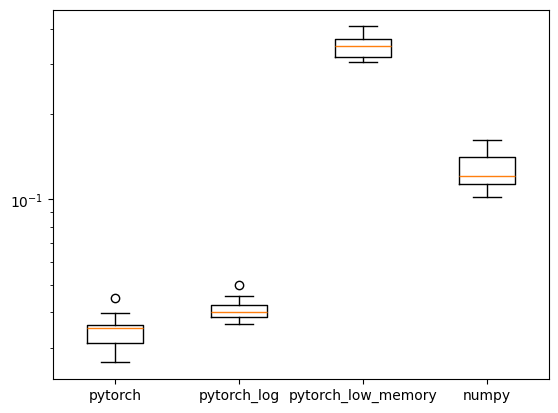
\includegraphics[width=0.8\linewidth]{speed_comparison_VEM.png}
    \caption{Speed comparison (in seconds) between implementations of the Variational EM algorithm for the mixture model. Each implementation was run 10 times, for 10 runs on a graph randomly generated using the SBM for 100 nodes and 3 classes.}
    \label{fig:speed_comparison}
\end{figure}

\bibliographystyle{abbrv}
\bibliography{bibliography}

\end{document}